\documentclass[12pt,letterpaper]{article}
\usepackage{times}
\usepackage[utf8]{inputenc}
\usepackage[spanish]{babel}
\usepackage{natbib}
\usepackage{amsthm,amsmath,amsfonts,amssymb}
\usepackage[doublespacing]{setspace}
\usepackage{threeparttable}
\usepackage{graphicx}
\usepackage{caption}
\usepackage{subcaption}
\usepackage{arydshln}
\usepackage{lscape}
\usepackage{pdflscape}
\usepackage{tabularx}
\setlength{\extrarowheight}{3pt}

\topmargin -1.5cm
\oddsidemargin 0.0cm
\textwidth 16.5cm 
\textheight 23cm
\footskip 1.0cm
\voffset 0cm

%\usepackage{setspace}
%\singlespacing
%\onehalfspacing
%\doublespacing
%\setstretch{1.1}

\title{Estimación de Tipo de Cambio Real de Equilibrio para Bolivia en el periodo 1999-2016} 

\author{Hugo Pablo Rocha Portugal \and Paola Cecilia Yujra Tonconi}

\date{}



%%%%%%%%%%%%%%%%% END OF PREAMBLE %%%%%%%%%%%%%%%%



\begin{document} 

\maketitle 

\begin{abstract}
jksajkdfjksdfkf
\end{abstract}

\newpage

\section{Introducción}

Tras la hiperinflación que Bolivia sufrió durante la primera mitad de los 80s, la economía local se restituyó caracterizada por la precariedad de sus mercados incluso habiéndose logrado una solución satisfactoria que puso fin a dicha patología en precios. La delicadeza de la situación estaba representada por un proceso de insipiente crecimiento debido a su economía primaria e informal que se vio combinada con régimen cambiario \emph{crawling peg}. Las constantes devaluaciones de la moneda local limitaron la efectividad de la política monetaria y generaron una alta dependencia al dólar americano. Al mismo tiempo, las condiciones particulares por las que la economía pasaba no permitieron cambiar su matriz productiva al paradigma industrial a diferencia de sus vecinos regionales que ya habían logrado incurrir en este camino décadas atrás; la explotación de materias primas para exportación aún constituía el factor de crecimiento característico de la economía boliviana, así como lo fue desde épocas coloniales. Como consecuencia de ello, el crecimiento económico en la década de los 90s fue limitado y caracterizado por una débil hegemonía institucional y política. Sin embargo, a mediados de la década de 2000s, el incremento de precios de materias primas sumado a la nacionalización de hidrocarburos se constituyeron en elementos claves para que Bolivia presente mejorías en sus indicadores macroeconómicos y sociales.

%Exito económico
El éxito de Bolivia en materia económica es sobresaliente desde 2004-2005 hasta la actualidad. Efectivamente, el país pasó de ser uno de los más pobres del subcontinente a tener el crecimiento económico más importante de la región. Al mismo tiempo, consiguió recaudar elevados niveles de Reservas Internacionales Netas, reducir los niveles de pobreza y desigualdad, des-dolarizar su economía, reducir los niveles de deuda y mantener niveles controlados de inflación. Incluso cuando los términos de intercambio no le favorecieron. A partir de 2014, Bolivia demostró una gran capacidad de resiliencia. Ante todos estos logros queda preguntarse cuales fueron los factores más importantes que contribuyeron a su consecución.

%Sector externo
Sin lugar a dudas, el desempeño de la balanza comercial se constituye en el influjo de divisas más grandes que Bolivia ha percibido en su historia. A partir de 2004 y consolidándose a finales de 2005, las exportaciones de hidrocarburos presentaron niveles elevados los cuales se incrementaban fuertemente periodo tras periodo. La consecuente nacionalización de 2006 fue una de las políticas nacionales más importantes pues permitió que el país capte, utilice y distribuya estas ganancias de la mejor manera que vio conveniente. Por estas razones, este fenómeno está altamente correlacionado con el citado éxito económico de los últimos 15 años. En este sentido, no es casualidad que la meta de las pasadas autoridades políticas y económicas del país haya estado orientada a la bonanza de comercio internacional basando sus esperanzas en el desempeño del sector extractivo.

En este periodo de boom, los impuestos directos a los hidrocarburos permitieron al gobierno central emprender políticas públicas importantes como la implementación de bonos sociales dirigidos principalmente a niños, madres en gestación y adultos mayores, los cuales constituyen la población más vulnerable del país. Asimismo, dichos influjos permitieron el incremento de RIN y gasto e inversión pública ejecutados a través del gobierno central así como por los gobiernos departamentales y municipales. Los proyectos públicos con mayor notoriedad que recibieron estos recursos son las Empresas Públicas Estratégicas, FINPRO, etc. Al mismo tiempo, estos recursos ejecutados en la economía permitieron a su vez el fomento del gasto e inversión privada magnificando los esfuerzos iniciales. Teóricamente, este contexto positivo dió curso a las condiciones que permitieron mantener el tipo de cambio nominal estable; lo cual tuvo como resultado la des-dolarización de la economía, el anclaje de las expectativas de la población sobre la moneda local y la reducción de presiones inflacionarias externas que permitió generar espacios para ejercer la política monetaria cuando fuese necesario. 

%TCR como nivel de competitividad
Debido a la importancia que las exportaciones tienen para la economía de Bolivia es pertinente estudiar aquellas variables económicas que la fomentan y los comovimientos que comparten. Si bien los términos de intercambio y la nacionalización de hidrocarburos beneficiaron al crecimiento, se deben identificar las políticas económicas que hayan incentivado el importante periodo de bonanza. En teoría, la más importante de ellas es el tipo de cambio real debido a que captura el nivel de competitividad de los productos bolivianos comparado con los de sus principales socios comerciales. La depreciación de esta variable implicaría el abaratamiento de los bienes y servicios nacionales haciéndolos más atractivos para su compra desde la perspectiva foránea; este hecho generaría el incremento de las exportaciones.

%Estabilidad cambiaria y como el TCN determina al TCR
Los hacedores de política fueron conscientes de la importancia del tipo de cambio real y de la bonanza en exportaciones. En efecto, el proceso cambiario de finales de los 80s hasta 2005 denominado \emph{crawling peg} se constituyó en la política cambiaria boliviana que tuvo como objetivo principal incrementar la competitividad nacional a través de constantes mini devaluaciones no anunciadas que, según el plan, permitirían mantener un tipo de cambio real consistente con un equilibrio en la balanza comercial. Sin embargo, a pesar del esfuerzo que implicó dicho régimen cambiario, no se logró el objetivo asumido sino hasta finales de su vigencia. De igual manera, llama la atención que el incremento de las exportaciones sucedió cuando el tipo de cambio real atravesó una fase de profunda apreciación implicando un hecho contrario a lo adelantado por la teoría.

%TCReq para saber cual es la mejor política cambiaria, cuanto cuesta mantener el tipo de cambio fijo y desalineamientos y como se mueve
En este marco, se propone estudiar el tipo de cambio real desde la perspectiva de su equilibrio. Esto permitiría encontrar el balance entre el denominado equilibrio interno y externo, Toda vez que los valores observados y los calculados de equilibrio determinan el desalineamiento al que se puede atribuir el desbalance reflejado en superávit o en déficit comercial. Al mismo tiempo, se puede concluir cual es la mejor política cambiaria para las circunstancias que atravesó el país. Mientras que desde un segundo enfoque, la estimación de este equilibrio cambiario, otorgaría información sobre el set de variables que llegan a determinarlo. 

%Lo que se encuentra en el paper
En este sentido, se utilizan dos metodologías convencionales y complementarias para calcular el tipo de cambio real de equilibrio, las cuales son BEER y DEER. La primera aproximación se enfoca en establecer los determinantes que se espera tengan efectos persistentes y de mediano plazo con el tipo de cambio real encontrado que el tipo de cambio real en tendencia se mantuvo en general bajo la senda de su equilibrio. La segunda metodología propone que los desalineamientos se encuentran antes de 2003 y después de 2013. El uso complementario de estas dos metodologías permiten entender que el primer modelo, más allá de determinar una senda de equilibrio que establece un equilibrio interno y externo, es útil para determinar cuales son las variables que afectan el movimiento de la variable en cuestión; asimismo, el segundo modelo permite entender el equilibrio de la variable en condiciones ``normales", sin embargo, a partir de un análisis más profundo, este método levanta sospechas sobre lo que realmente pasó en la economía boliviana durante los años de bonanza que permitieron que la economía goce del \emph{momentum} necesario para lograr el destacable desempeño referido previamente.

Este documento encuentra que las variables que explican los incrementos de exportaciones y balanza comercial son el incremento de términos de intercambio; el éxito económico derivado de este fenómeno es maximizado por la consecuente nacionalización de hidrocarburos que permite que el gobierno tenga hegemonía sobre los recursos generados por dicha circunstancia. El incremento de precios de hidrocarburos es independiente de las políticas bolivianas, mientras que la nacionalización es una política interna exógena. Asimismo, el tipo de cambio real no es una medida de competitividad para la mayor parte de bienes que Bolivia exporta, por tanto, su apreciación no la deteriora. Por otro lado, el tipo de cambio real es una medida adecuada de competitividad para las importaciones, su apreciación se puede entender como un factor que, junto al crecimiento económico del país, ayudó a fomentarlas sin perjudicar los elevados valores de exportaciones. A pesar de este último comportamiento, se identifica una baja sensibilidad de las importaciones frente el tipo de cambio real, esta inelasticidad puede ser explicada por la baja capacidad de sustitución de importaciones que la producción boliviana ofrece al consumidor en términos de bienes finales. En este sentido, el tipo de cambio real no es una medida certera de competitividad así como puede ser caracterizada por una medida de poder de compra de la moneda boliviana.


%El régimen cambiario boliviano fue mutando a través del tiempo. Para acabar con el proceso hiperinflacionario de 1984-1985 se instauró el Bolsín, mecanismo por el cual se reunificaron los tipos de cambio oficial y paralelo permitiendo así la convertibilidad libre de la moneda nacional. Este mecanismo fue mutando hasta constituirse en el régimen \emph{crawling peg} caracterizado por mini devaluaciones controladas y periódicas (reptantes) cuyo objetivo nominal era mantener la competitividad nacional frente el comercio internacional. A partir del 2005, se suscitó un periodo de apreciación que se agudizó entre 2007 y 2008 hasta que en comienzos de 2009 se optó por la estabilidad cambiaria, únicamente seguida por leves apreciaciones en 2010 y 2011. Dicha estabilidad cambiaria continúa hasta la actualidad consituyéndose en el ancla nominal de expectativas a la que se atribuye el principal rol de control de la inflación al limitar las presiones inflacionarias externas y permitió la notable des-dolarización que la economía ha experimentado, gracias a la cual la política monetaria es capaz de cumplir con su objetivos.

%La contraparte real del tipo de cambio tiene un comportamiento más volátil que la variable nominal, sin embargo, se puede distinguir claramente una tendencia de depreciación y apreciación entre los años 1999 y 2016. El incremento del indicador se extiende hasta finales de 2006 y da pié a una profunda apreciación. Existen dos grandes caídas en el indicador en 2002 y 2008 que corresponden por las crisis de Argentina y la crisis financiera internacional, respectivamente. En los últimos diez años, el contexto internacional al que Bolivia se vio expuesto estuvo protagonizado, en un primer periodo, por el boom de precios de materias primas que implicó el fortalecimiento de Bolivia y de los países socios comerciales generando ingresos altos por exportación a través de una fuerte y sostenida demanda externa. Cuando estos precios cayeron en 2013-2014, las economías circundantes entraron en un periodo de desaceleración e incluso, sumando otras factores internos, de recesión que implicó la depreciación nominal conjunta\footnote{Nótese que los regímenes cambiarios de las monedas latinoamericanas tienden a ser flotantes para absorber los impactos de los shocks externos de precios.} de sus monedas con niveles de inflación considerablemente elevados. %En contraposición, desde 2005 Bolivia demostró poder controlar paulatinamente las presiones inflacionarias externas que coincide con la apreciación real de su moneda hasta mediados de 2016, mostrando un manejo efectivo de su política monetaria en condiciones externas desfavorables. 

%Durante los últimos trece años Bolivia consiguió un crecimiento económico destacable a pesar que entre 2012 y 2015 el contexto internacional se tornó gradualmente más adverso y recién en 2016 y comienzos de 2017 se produce una normalización de las economías internacionales. A través de estos años, el comportamiento del tipo de cambio real, nominal y los beneficios económicos no parecen presentar una relación causal normal. La teoría indica que la fuerte y sostenida apreciación real debería haber perjudicado la cuenta corriente boliviana desde 2005 hasta 2012, al mismo tiempo, la pequeña economía boliviana en desarrollo, después de verse concluido el periodo de boom de materias primas, debería haber sido arrastrada por la tendencia de desaceleración y crisis económica regional que derivó en depreciaciones colectivas, sin embargo, la realidad demuestra una situación distinta. Mucho de este éxito ha sido oficialmente atribuido a las políticas económicas contracíclicas, a la demanda interna y a la significativa exportación del gas que actuaron conjunto a la política cambiaria heterogénea.

%En un contexto en el que el papel del sector externo de la economía boliviana es importante, especialmente debido al rol protagónico de la exportación de hidrocarburos, se debe evidenciar y analizar las medidas esgrimidas en los periodos analizados especialmente los referidos a la política cambiaria que determinan, en sincronía con el contexto político, las condiciones y ambiente relevante para el desarrollo económico boliviano. Para tal efecto, el nivel de tipo de cambio real de equilibrio, a partir del cual se calculan los desalineamientos del efectivo, es una herramienta a partir de la cual el debate sobre la pertinencia de la política cambiaria en el pasado, presente y futuro del país cobra relevancia. 

%Para motivar esta necesidad de estudio se debe notar que el nivel del tipo de cambio nominal era determinado por la ``regla cambiaria'' que implicaba mantener el nivel de tipo de cambio real en un punto en el que la balanza comercial esté en equilibrio.\footnote{La regla cambiaria y estimación del tipo de cambio de referencia es derivado de la definición del tipo de cambio real en la que $E_t^r=\bar{Q}_{2003}\frac{P_t}{P_t^*}$ donde para el cálculo expuesto en la figura \ref{tcn}, $\bar{Q}_{2003}=100$ y corresponde al año 2003 en el periodo en el que se alcanza equilibrio de la balanza comercial} La figura \ref{tcn} muestra al tipo de cambio, de aquí en adelante, de referencia o referencial que mantiene fijo al tipo de cambio real con base 2003.\footnote{Claramente, no se pretende inferir que en los 90's los tomadores de decisión utilizaban esta variable con año base 2003, pero cualquier otro año base, en especial de algún momento en el que la balanza comercial haya estado en equilibrio, generaría resultados similares.} Se pueden distinguir dos momentos importantes del periodo citado, el primero se constituye en el seguimiento de dicha regla cambiaria y el segundo está caracterizado por la estabilidad cambiaria definiendo como punto de inflexión entre ambos al año 2008. 

%\begin{figure}
%\centering
%\caption{Tipo de cambio nominal y su referencia}\label{variables}
%        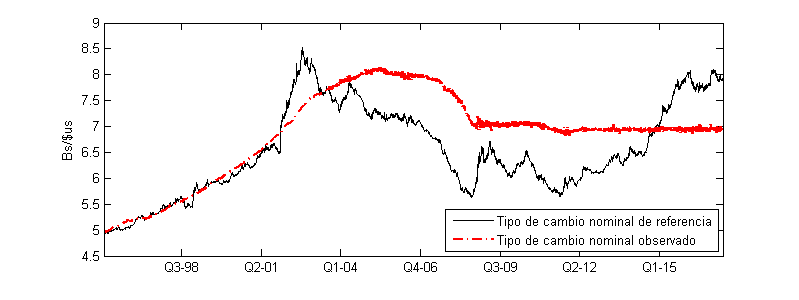
\includegraphics[width=\textwidth]{tcn}
%        \label{tcn}
%\end{figure}

%En efecto, hasta casi finales de 2008 el tipo de cambio nominal fue determinado siguiendo el movimiento de su referencial exceptuando el momento en el que la crisis económica de Argentina generó presiones de depreciación en esta variable.\footnote{Desde la perspectiva de la regla cambiaria siguiendo el tipo de cambio referencial, los tomadores de política interpretan los picos generados por las crisis como pasajeros y deciden no seguirlos, mas bien parecen continuar con la tendencia previa hasta ya pasados los efectos de la crisis. Específicamente, durante la crisis Argentina de 2002 que chocó fuertemente a Bolivia, los tomadores de decisión bolivianos decidieron continuar con una leve depreciación en niveles ya determinados que se prolongó hasta pasada dicha crisis.} Como ha sido ya mencionado, después de mediados de 2003 Bolivia consiguió el equilibrio de su balanza comercial que sería seguido por un ciclo de superávits. Durante este periodo se genera un comportamiento de ``u'' invertida del tipo de cambio nominal que parece indicar que los tomadores de decisión buscaron retomar la regla cambiaria en una situación en la que el tipo de cambio nominal y de referencia se encontraban desalineados. El \emph{catching up} de dicha variable se dio a mediados de 2008. En el cuarto trimestre del mismo año, afrontando la crisis financiera internacional, Bolivia decide mantener su tipo de cambio nominal constante, interpretando el cambio de dirección sugerido por la crisis como transitorio. A pesar que durante 2011 se aprecia levemente la moneda boliviana, la regla cambiaria que buscaba conciliar los tipos de cambio nominal y referencial es abandonada a pesar de que este último sugería la depreciación sostenida, el cual es el comportamiento que la mayoría de las economías de la región presentaron en dicho periodo.

%Este cambio de dirección de la política cambiaria implicó la notable des-dolarización de la economía boliviana, debido a que permitió cambiar las expectativas que la población tenía con respecto al tipo de cambio nominal. Previo a 2005, el régimen de \emph{crawling peg} permitía a la población esperar que el boliviano se devalúe constantemente, en una economía pequeña y altamente dolarizada esto implicaba una perdida constante del poder de conservación de valor de la moneda nacional y sugería al dólar americano como principal instrumento financiero y fiduciario para conservar riqueza e incluso efectuar transacciones monetarias grandes. Desde finales de 2008, los efectos de la significativa apreciación fueron evidentes, estos implicaron que la moneda boliviana podía no solo mantener valor sino también generarlo frente al dólar americano, la principal divisa en el mundo. La posterior estabilidad cambiaria implicó el anclaje de la expectativa del valor del boliviano que junto a otras medidas adyacentes contribuyeron a que sea la principal moneda circulación en Bolivia para el ahorro, crédito y transacciones monetarias. Al no depreciarse constantemente, los precios de bienes importados y derivados de los mismos dejaron de inflarse por efecto de dicho efecto cambiario dando espacio de acción a la política monetaria doméstica. Además, el rendimiento del comercio externo demostró buenos resultados con la inducción de esta política heterodoxa.

%La regla cambiaria utilizada basada en el tipo de cambio de referencia sugiere que Bolivia tiene como objetivo de política cambiaria mantener la competitividad del sector externo y que el tipo de cambio es uno de los instrumentos para lograrlo. Sin perdida de generalidad se puede observar que este ha sido un paradigma importante de política económica en Bolivia siempre buscando generar el valor agregado y captación de divisas a través del fomento de las exportaciones. La bonanza de la economía boliviana de los últimos años ha demostrado que su salud depende de su posición acreedora en la balanza comercial. Estas evidencias delimitan una serie de cuestiones importantes en el tema de efectividad de las políticas económicas llevadas a cabo. ¿Es el tipo de cambio real de equilibrio aquel que determina el balance entre las exportaciones e importaciones?. ¿Cuál es el tipo de cambio real que permite la consecución de este objetivo?. ¿Es el tipo de cambio nominal el instrumento efectivo que permite el movimiento del tipo de cambio real?. 

%Son estas las cuestiones que motivan el análisis de la política cambiaria boliviana y muy en especial la tendencia de equilibrio del tipo de cambio real del país. A continuación, se estima y analiza bajo los métodos de BEER y una variación de FEER (DEER) las medidas de TCR de equilibrio de corto y mediano plazo. No se realiza el análisis de largo plazo porque es considerado poco significativo para la economía boliviana que aún se encuentra en vías de desarrollo y donde aún no se tiene indicios claros del camino de desenvolvimiento pertinente que contribuya a su crecimiento sostenido y sustentable siendo este último la senda de \emph{steady state} en \emph{stricto sensu} que no es aún vislumbrada. Asimismo, se discute ideas centrales de política cambiaria, se plantean posibles desaciertos, miopía conceptual y se introduce la idea de subvaluación estructural de la moneda en una economía determinada por un fuerte contrabando (importaciones ilegales).

Bajo esta motivación el presente documento plantea la consideración de elementos importantes como definiciones e intentos previos de medir el tipo de cambio real en Bolivia en la sección \ref{pre}; posteriormente, se define la metodología y marco de medición en la sección \ref{tcr}; la verificación de series estadísticas, hechos estilizados y resultados son planteados en la sección \ref{calc}; se continúa con conceptos e ideas teóricas inspiradas en la realidad boliviana en la sección \ref{consid} y para sintetizar lo estudiado la sección \ref{concl} finaliza con las reflexiones más importantes del documento.



\section{Revisión de Literatura}\label{pre}

\subsection*{Definiciones y consideraciones}
%TCR
El tipo de cambio real es la variable que refleja cuanto de una canasta básica doméstica es necesaria para comprar una canasta básica extranjera. Esta variable es determinada por la siguiente relación:
\begin{equation}\label{tcr1}
Q_t=E_t\frac{P_t^*}{P_t},
\end{equation}
donde $Q_t$ es el tipo de cambio real, $E_t$ es el tipo de cambio nominal, $P_t^*$ representa el índice de precios de una canasta básica representativa de una economía extranjera y $P_t$ es el índice de precios de una canasta básica doméstica representativa. En logaritmos la expresión \ref{tcr1} es representada por:
\begin{equation}\label{tcrlog}
q_t=e_t+p_t^*-p_t.
\end{equation}
Nótese que las minúsculas describen a la variable en logaritmo. Tanto las expresiones \ref{tcr1} y \ref{tcrlog} representan el poder de compra de una moneda frente a otra. El tipo de cambio real también puede ser analizado en términos de precios transables y no transables.\footnote{En realidad, todas expresiones procuran medir la siguiente relación original de tipo de cambio real medida entre precios no transables y transables $Q_t=\frac{P_{NTt}}{P_{Tt}}$.} Para tal efecto, en el caso de \ref{tcrlog} se asume que $p_t=\alpha p_{Nt} + (1-\alpha)p_{Tt}$, donde $0<\alpha<1$, $\alpha=\alpha^*$, en este contexto, $p_{Nt}$ es el precio de no transables, $p_{Tt}$ el de transables y $\alpha$ es la proporción de precios de bienes no transables que constituyen el índice de precios. Entonces:
\begin{equation}\label{tcr2}
q_t=q_{Tt}+\alpha(\hat{p}_{Nt}-\hat{p}_{Tt}),
\end{equation}
donde, el circunflexo implica la diferencia de la variable entre precios domésticos y extranjeros, por ejemplo $\hat{p}_{Nt}=p_{Nt}^*-p_{Nt}$, y $q_{Tt}$ es el tipo de cambio real de bienes transables donde $q_{Tt}=e_t+p_{Tt}^*-p_{Tt}$. Por lo general, se asume que $q_{Tt}=0$ (o $Q_{Tt}=1$) debido a que los precios transables podrían ser los mismos tanto en la economía doméstica como en el exterior, de esta manera su comercialización en los mercados internacionales hace que tengan los mismos precios alrededor del mundo. 

Las ecuaciones \ref{tcr1} y \ref{tcrlog} son análogas e implican que, manteniendo todo lo demás constante, los incrementos de tipo de cambio nominal (devaluación nominal) o de los precios extranjeros o las caídas del nivel de precios local determinan una depreciación real de la moneda nacional. Lo contrario aplica para el caso de una apreciación real. Sin embargo, desde la perspectiva caracterizada en \ref{tcr2}, el tipo de cambio real de bienes transables y la diferencia del nivel de precios no transables, y transables, entre el resto del mundo y la economía local determinan los movimientos de la variable en cuestión. Esta última descripción implica una perspectiva más operativa debido que a partir de ella se puede distinguir cual es el efecto de las políticas económicas sobre cada conjunto de bienes. El caso más estudiado, y que empíricamente tiene mayor soporte en la literatura abocada a calcular el equilibrio de tipo de cambio real, entiende que el gasto público (política fiscal) es orientado en su mayoría en bienes no transables, este incremento de demanda permite que los precios de estos bienes se incrementen. 

Por otro lado, la teoría contemporánea no describe cual es el efecto de las otras políticas económicas sobre cada conjunto de bienes. Sin embargo, a continuación se ensayan algunas consideraciones al respecto. El impulso de la política monetaria (sin tomar en cuenta los efectos asimétricos sobre el nivel de precios) afecta en mayor medida a los precios no transables, como servicios y bienes locales cuyos precios dependen del dinamismo de la economía nacional y la inflación. En contraposición, los niveles de precios transables son determinados en mayor medida por los mercados internacionales. En consecuencia, dentro del territorio nacional el nivel de precios transables importados con precios en moneda doméstica serían más influenciados por las depreciaciones de la moneda local (política cambiaria); los niveles de precios de bienes transables producidos domésticamente estarían afectados por el nivel de costos de trabajo e insumos locales y de procedencia extranjera sobre los cuales la política cambiaria también tiene influencia. Asimismo, se entiende que la competencia entre bienes transables locales e importados es importante en la determinación de precios finales en la economía. Se retomará esta discusión en la sección \ref{consid}.

Es importante destacar que en la teoría económica moderna se entiende que la política económica no tiene influencia en el cambio de tendencia del equilibrio de largo plazo del tipo de cambio real. Esto porque, dados los niveles de los fundamentos, la tendencia y el equilibrio están dados. En contraposición, el papel de la política económica está orientada en influir a los fundamentos para que el tipo de cambio real retorne a su nivel de equilibrio cuando se encuentre desequilibrado. Esta perspectiva implica que no se puede estar desviado del nivel de equilibrio por mucho tiempo. Sobre como influir en el movimiento del tipo de cambio real se ampliará la discusión en la sección \ref{consid}.

Entonces, como se ha anotado previamente, las representaciones del tipo de cambio real \ref{tcrlog} y \ref{tcr2} son importantes por distintas razones. La primera, que está basada en el propio concepto de la variable, es utilizada para construir estadísticamente el indicador pertinente que caracteriza dicha variable. Por otro lado, la segunda expresión permite realizar una interpretación sobre las fuerzas que podrían influir en sus movimientos.

Hay algunas consideraciones prácticas al respecto del tipo de cambio real que deben ser apuntadas. En particular, $p_t^*$ y $p_t$ no siempre representan precios de las mismas canastas básicas, esto porque distintos países consumen distintos bienes básicos, o en otras palabras, no todas las economías incluyen exactamente los mismos productos en sus canastas, adicionalmente, esto se puede deber a que frente la modernización y aparición de nuevos bienes, los institutos de estadística tardan en actualizar los productos que deberían entrar en la canasta básica. En teoría, esto podría ocasionar algún ruido en el cálculo del tipo de cambio real que en promedio puede asumirse insignificante, aunque queda la duda hasta qué punto esto es perjudicial.\footnote{Por ejemplo, ¿es relevante entre 2010-2017 incluir los servicios de telefonía pública (cabinas fijas y ambulantes), videoreproductor, VHS, minicomponente, walkman, discman y tantos otros dentro de la canasta básica?} Por otro lado, cuando se relaciona al TCR con el comercio internacional de, por ejemplo, materias primas, parece que esta medida cambiaria no tiene incumbencia pues, como ha sido expuesto, mide la relación de bienes que entran dentro de la canasta básica, a la cual las materias primas y demás insumos productivos son ajenos pero altamente comercializados internacionalmente. Finalmente, a pesar que algunos investigadores asumen que $q_{Tt}=0$, debido al supuesto de perfecta sustitubilidad de bienes transables, en este documento se considera importante tomar en cuenta la diferenciabilidad horizontal y vertical de bienes transables.

%TCReq
Dada la definición del tipo de cambio real es preciso establecer la definición de su correspondiente equilibrio. El mismo es una variable no observada que idealmente podría ser considerada como el contrafactual positivo\footnote{Desde la perspectiva deontológica de la ciencia.} del tipo de cambio real. En otras palabras, es la variable que captura los valores ideales o en equilibrio de los componentes que conforman el tipo de cambio real. En este sentido, se entiende como valor de equilibrio al tipo de cambio real que representa a la economía abierta que está en equilibrio tanto a nivel interno como externo. Las implicaciones de lo que implica estar en equilibrio son discutibles porque implica distintas interpretaciones dependiendo de la perspectiva del autor.

El propio hecho de que una variable denominada tipo de cambio real de equilibrio exista, indica que la ciencia social acepta tanto teórica como empíricamente que el tipo de cambio observado no está conformado por los valores de equilibrio de los mercados pertinentes que lo conforman. En este sentido, se puede entender que existen distorsiones (transitorias o inesperadas) en dichos mercados que generan valores observados que podrían no corresponder a lo que deberían representar y en el peor de los casos retroalimentarse debido a algún tipo de persistencia. El hecho de reconocer este hecho permite entender a las distorsiones transitorias o no anticipadas desde distintos puntos de vista, lo cual da pié a tener varios tipos de conceptos de equilibrio.

%Eq CP MP LP
Bajo esta premisa, \cite{driver2005concepts} distingue tres tipos de conceptos centrales de equilibrio utilizados y operativizados por distintos autores. Los de corto plazo que capturan movimientos de la serie correspondientes a los de sus fundamentos y a factores transitorios abstrayendo únicamente los shocks inesperados. Los de mediano plazo que se caracterizan por su compatibilidad con el balance externo e interno de la economía, es decir, esta perspectiva es consistente con los fundamentos en su nivel tendencial, los mismos que pueden estar aún convergiendo, o no, a sus valores de estabilidad de largo plazo. Y, finalmente, el equilibrio de largo plazo ocurre en pleno empleo y es compatible con los co-movimientos de los valores de largo plazo de sus fundamentos, en otras palabras, cuando no hay cambio endógeno de tendencia.

El concepto de equilibrio de corto plazo implica que los mercados están en equilibrio pero son afectados por impulsos transitorios y shocks inesperados. La remoción de estos últimos elementos constituye el objetivo operativo de estos modelos para encontrar el equilibrio. El concepto de mediano plazo, asume que los datos observados podrían no corresponder al equilibrio en los mercados que los generan; para contrastar esta hipótesis, encuentra la diferencia entre los niveles, que asume, de equilibrio del sector interno y externo y los compara con los niveles tendenciales de las variables observadas. Finalmente, el concepto de largo plazo implica que todos los mercados deberían estar en pleno empleo y en total equilibrio, entonces, a partir de los datos observados se construye una estructura de la economía que aproxima las interelaciones de las variables capaces de reproducir su pleno empleo.

%Eq interno externo
Entonces, asumir que el mercado interno y externo están siempre en equilibrio y los datos observados son una reproducción de dicha relación implica un supuesto importante para determinar el concepto de equilibrio que vaya a ser ejercitado. En tal sentido se propone utilizar ambas nociones, una que asuma que los mercados efectivamente están siempre en equilibrio y otra que asuma la existencia de un equilibrio más allá de lo observado.

Con respecto a la perspectiva de largo plazo en la que los valores que se deben utilizar para encontrar la senda de equilibrio son los de \emph{steady-state} y pleno empleo, se debe establecer las siguientes consideraciones. Dichos resultados de pleno empleo son obtenidos en base a valores pasados y realizaciones económicas actuales que supondrían un crecimiento vegetativo bajo un esquema y estructura de la economía determinado por las relaciones actuales. En tal sentido, es primordial tener una estructura que esté bien realizada, generalmente, cuando se utilizan identificaciones para países desarrollados con datos de países en desarrollo esto puede implicar un error debido a que distintos países tienen características distintas que pueden y deben ser incluidas. Por otro lado, estos modelos de largo plazo implican que se caracterice a la economía en cuestión en \emph{steady-state} y pleno empleo convergiendo a su equilibrio de largo plazo. Este puede ser un concepto adecuado para países desarrollados, pero no para países en desarrollo que no tienen una estructura económica consolidada y que tiene razones para considerar cambiarla y mejorarla. Bajo este último criterio y en estas economías, el equilibrio de largo plazo no se vislumbra a partir de los datos observados. 

A partir de estas consideraciones y en aras de determinar la metodología para medir el tipo de cambio real de equilibrio para realizar el análisis que compete, se plantean los siguientes objetivos. En primer lugar lugar, determinar si el tipo de cambio real de equilibrio es realmente aquel que permite el balance comercial. En segundo lugar, se pretende estimar cuales son las fuerzas económicas que mueven el valor de tipo de cambio real. 
Los objetivos delineados previamente implican observar conceptos de corto y mediano plazo. Asimismo, servirán para dar explicación a otras cuestiones importantes.



\subsection*{Importancia del equilibrio}
%Por qué es necesario medir el equilibrio
La literatura especializada en la determinación de un tipo de cambio real de equilibrio es vasta y reúne una variada cantidad de definiciones, métodos y consideraciones especiales al respecto. Por ejemplo, \cite{driver2005concepts} propone que una de las razones más importantes por las cuales determinar dicho equilibrio es para que economías con tipos de cambio poco flexibles determinen el costo de mantener esta variable relativamente fija. Adicionalmente, realizar el cálculo permitiría entender cuales son los principales \emph{shocks} externos que mueven la trayectoria de la variable fuera de su equilibrio y cuales son las variables que influyen en su movimiento \citep{macdonald2000concepts}. Esta perspectiva está basada en el supuesto de que economías con tipo de cambio flexible estarían siempre alrededor de su valor real de equilibrio por estar definidas libremente en sus mercados mediante el equilibrio de los mismos. Por otro lado, la importancia conceptual de representar el equilibrio tanto interno como externo permitiría verificar la fortaleza de la moneda tanto local como internacionalmente \citep{akrama2003real}.

\subsection*{Metodologías}
%Basado en los surveys corto conciso y finalmente analítico concentrarse no en describirlos pero en los pros y contras
Para definir la metodología de medición es necesario determinar cual es el objetivo final de la derivación del tipo de cambio real de equilibrio. Como ha sido adelantado, hay una variedad de métodos de los cuales se puede escoger dependiendo de la finalidad y alcance que se quiere dar a la perspectiva de estudio. \cite{driver2005concepts}, \cite{macdonald2000concepts} e incluso \cite{akrama2003real} ofrecen una buena recolección de métodos.

Los equilibrios obtenidos de estas metodologías son distintos entre ellos. La razón se basa en el hecho que cada una está determinada por diferentes supuestos y conceptos de equilibrio. Como se ha decidido revisar una visión de completariedad entre el corto y mediano plazo se procederá a revisarlas y escoger a la que se constituya la más apropiada desde la perspectiva económica de Bolivia.

En el corto plazo se distingue particularmente los métodos de PPC y BEER. El primero está basado en el cumplimiento de la condición de poder de paridad de compra. Sin embargo, esta alternativa no es realista debido a que no existe la completa flexibilidad de precios que permita que la condición se cumpla a cabalidad existiendo bloqueos y distorsiones estructurales a través de impuestos y aranceles, por otro lado, también se puede citar la diferenciación horizonal y vertical como una razón por la que esta condición no se cumpla. Adicionalmente, el efecto \emph{Balassa-Samuelson} propone que el efecto de los precios descompuestos entre transables y no-transables \citep{balassa1968effective} es importante en la definición del tipo de cambio real, mientras que a través de esta perspectiva no se observa dicha caracterización. Trabajos empíricos indican que de cumplirse, esta relación lo haría en el largo plazo. Confirmando el rechazo de esta hipótesis, investigaciones empíricas en Bolivia como \cite{lora2000tipo} y \cite{humerez2005reexaminando} descartan su aplicación.

La siguiente alternativa es el modelo BEER (\emph{behavioral equilibrium of exchange rate}) que se basa en determinar el equilibrio de tipo de cambio comportacional determinado por sus fundamentos. Este modelo es asociado con el trabajo de \cite{clark1999exchange}. La idea es establecer la relación de cointregración entre el tipo de cambio real y sus fundamentos, dado que estas variables al ser integradas en primer grado comparten una relación de largo plazo que es implementada por un modelo de corrección de errores que mide de los efectos de corto plazo de las variables. Asimismo, este modelo permite determinar como es que los fundamentos explican los movimientos de corto plazo en la relación de equilibrio.

Esta será la perspectiva de corto plazo que se utilizará para hallar el tipo de cambio real de equilibrio. La identificación original de \cite{clark1999exchange} se basa en el cumplimiento de la paridad encubierta de tasas de interés, sin embargo, hay otros tipos de identificación que desembocan a estimaciones similares.

Con respecto al equilibrio de mediano plazo se analizan las principales opciones determinadas por la literatura. En esta línea existen dos corrientes de estimación con sus respectivas variantes. En primer lugar, los modelos de equilibrio permanente, y en segundo lugar, los de equilibrio de fundamentos. Estos últimos implican un balance tanto interno como externo con el cual determinan una trayectoria de tendencia normativa de la economía. Típicamente son conocidos como FEER. En segundo lugar están los modelos PEER y APEER que según \cite{driver2005concepts} son métodos que pueden ser entendidos como de largo plazo y más estadísticos que económicos, por esta razón se decide enfocarse simplemente en los de la familia FEER (\emph{fundamental equilibrium of exchange rate}).

El equilibrio en los modelos FEER ocurre cuando cierto nivel de tipo de cambio real permite el logro de los niveles de cuenta corriente norma y PIB en sus niveles de tendencia, de esta manera, se consigue el equilibrio interno y externo. Existe una variedad de métodos de estimaciones FEER, las mismas se diferencian en sus maneras de establecer la mejor forma de conciliar el equilibrio externo con el interno haciendo uso de las distintas normas de cuenta corriente y valores subyacentes, entre estos se puede distinguir el balance macroeconómico y la sostenibilidad externa \citep{bussiere2010methodological}. Por otro lado, una perspectiva más flexible de FEER permite al investigador determinar los niveles deseados de cuenta corriente y PIB de acuerdo a los objetivos políticos de un país, este método es conocido como DEER (\emph{desired equilibrium of exchange rate}).

Asimismo, el uso de componentes de norma y subyacente para FEER implican asumir supuestos y adoptar como meta de equilibrio económico las condiciones que el balance macroeconómico y la sostenibilidad externa proponen. Por esta razón y porque se conocen los objetivos de política cambiaria se encuentra conveniente utilizar DEER. Hay dos metas que los hacedores de políticas bolivianos han tenido desde 1985, estas son limitar la variabilidad del producto permitiendo una tendencia de crecimiento positiva y sostenida y que la balanza comercial presente equilibrio o en el mejor de los casos superávit caracterizando de este modo una cuenta corriente positiva.

Entonces, dado el repaso de las metodologías existentes y tomando en cuenta la pertinencia de ellas para su aplicación en el caso boliviano, se aplicará la metodología BEER y DEER para realizar la estimación del tipo de cambio real de equilibrio. 

\subsection*{Evidencia empírica internacional}
%La mayoría de esta literatura no solamente es el paper teórico sino tambien la aplicación
%Países desarrollados
%Países emergentes
%Países en desarrollo
%Países de la región


\subsection*{Evidencia empírica en Bolivia}
%Qué se ha hecho
Acompañando la búsqueda del cometido que se tiene en el presente documento se ha revisado la evidencia de investigaciones en Bolivia en la búsqueda de la determinación del tipo de cambio real de equilibrio. En tal sentido se hace referencia a \cite{ferrufino1992tipo}, \cite{aguilar2003estimacion}, \cite{humerez2005reexaminando}, \cite{montiel2007equilibrium}, \cite{cerutti2008}, \cite{mendieta2008equilibrio}, \cite{bello2010tipo}, \cite{cerezo2010desempeno} y \cite{cerezo2011tipo}. Existen grandes similitudes entre todas las investigaciones generadas especialmente después de 2000. En primera instancia todos buscan estimar los desalineamientos con respecto al equilibrio, y en segundo lugar, todos presentan una metodología similar.

%Metodología + resultados importantes
En este sentido, los documentos citados se diferencian por su identificación a pesar que en última instancia ejecutan la misma metodología econométrica. Típicamente, los documentos que presentan estructura de identificación son aquellos previos al 2005. Específicamente, se hace referencia a la identificación de \cite{lora2000tipo}, citada también por \cite{aguilar2003estimacion} la misma que se constituye en la principal sistematización teórica que justifica el comportamiento del tipo de cambio real. Esta identificación está basada en el trabajo analítico de \cite{hinkle1999exchange} que asocia la demanda de trabajo en los sectores transables y no transables de una economía y la producción generada por los mismos junto con los componentes de la cuenta corriente y el comportamiento del gobierno. Adicionalmente, \cite{humerez2005reexaminando} utiliza la identificación de \cite{elbadawi1994estimating} a partir de las identidades y relaciones de cuentas nacionales. 

Los documentos posteriores no presentan claramente una estrategia de identificación, sin embargo, heredan el método de cointegración original y se concentran en probar la inclusión de distintos fundamentos en la relación de estudio y ampliar la base de datos, siendo que esta última no está unificada entre las investigaciones analizadas. Por este motivo, es que se puede concluir que para estos trabajos la identificación del movimiento del TCR determinado por sus fundamentos es no estructural. Al mismo tiempo se podría proponer que siguen una visión de estimación reducida, que es como puede ser identificada estas metodologías en la literatura pertinente.

Entre estos trabajos se debe destacar a \cite{cerezo2011tipo} que además del acostumbrado modelo de comportamiento de fundamentos (BEER) adiciona otras perspectivas analíticas más que le permiten estimar distintas trayectorias de equilibrio del TCR: el método de equilibrio macroeconómico, de sostenibilidad externa, un modelo que procura calcular el efecto Penn Balassa Samuelson y un modelo de equilibrio general. 

Los primeros dos métodos adicionales del documento citado de \cite{cerezo2011tipo} en realidad corresponden a distintas mediciones del balance externo de la economía norma correspondiente al método FEER como puede constatarse en \cite{bussiere2010methodological}.\footnote{A pesar de que \cite{bussiere2010methodological} exponen los métodos para calcular la cuenta corriente norma que pertenecen a la familia de métodos FEER, la principal fuente metodológica de \cite{cerezo2011tipo} es \cite{isard2007equilibrium}} Estos no ofrecen una perspectiva para todo el periodo de tiempo considerado, únicamente para el año 2010 para el que determinan una subvaluación de 1\% y 0,8\% para los métodos denominado equilibrio macroeconómico y sostenibilidad externa, correspondientemente. De la misma manera el modelo que estima el efecto Penn Balassa Samuelson (que es un efecto Penn de sección cruzada) es ejecutado para calcular una subvaluación de 16\% para el año 2010. Mientras que con los restantes dos métodos (BEER y DSGE) consiguen determinar una serie para el TCR de equilibrio durante el periodo para el que tienen datos. A propósito del modelo DSGE, se aduce una identificación basada en el modelo escandinavo de inflación, los modelos intertemporales de los 80's y la literatura de los ciclos reales.

%\begin{landscape}
\begin{table}
\begin{center}
\caption{\centering Lista de Fundamentos de TCR incluidos en estudios para Bolivia y signo con el que intervienen en la relación}
\begin{threeparttable}
\resizebox{\textwidth}{!}{ 
\begin{tabular}{lccccccccc}									
\hline
\hline													
Estudio	&	 Lora	&	 Aguilar	&	 Humerez	&	 Montiel	&	 Mendieta	&	 Cerutti	&	 Bello	&	 Cerezo	&	 Cerezo	\\

	&	 2000	&	 2003	&	 2005	&	 2007	&	 2008	&	 2008	&	 2010	&	 2010	&	 2011	\\
	
\hline										
Años de estudio	&	 1988-1999	&	 1990-2002	&	 1990-2003	&	 1969-2005	&	 1991-2007	&	 1990-2006	&	 1969-2006	&	 1992-2009	&	 1990-2010	\\

Periodicidad	&	 Trimestral	&	 Trimestral	&	 Trimestral	&	 Anual	&	 Trimestral	&	 Trimestral	&	 Anual	&	 Trimestral	&	 Trimestral	\\

\hline
 Gasto público	&	-	&	-	&		&		&	+	&	+	&		&	+	&	+	\\
\hline
 Términos de intercambio	&	-	&	-	&	-	&	-	&	-	&	-	&	-	&	-	&	-	\\
\hline
 Política Comercial	&	-	&	+	&		&		&	-	&		&		&		&		\\
\hline
 Balanza Comercial	&		&		&		&		&	-	&		&		&	+	&	-	\\
\hline
 Flujos de Capital	&	-	&	-	&	+	&		&		&	-	&		&		&		\\
\hline
 Apertura Comercial	&	+	&	+	&	+	&		&		&		&	+	&		&		\\
\hline
 Diferencial de tasas de interés	&		&	-	&		&		&		&		&		&		&		\\
\hline
 Productividad	&		&		&		&	-	&	+	&	-	&		&		&		\\
\hline
 Libor	&		&		&	+	&		&		&		&		&		&		\\
\hline
 Dummy (94-95)	&	+	&	+	&		&		&		&		&		&		&		\\
\hline
 IPC externo	&	+	&		&		&		&		&		&		&		&		\\
\hline
 Precio del Gas	&		&		&		&		&		&		&		&		&	-	\\
\hline
 RIN	&		&		&		&		&		&		&		&		&	-	\\
\hline
 NFA	&		&		&		&		&		&	-	&		&		&		\\
\hline
Sobrevaluado	&	 98-99	&	 90-93, 97-99	&	 91-93, 98-00, 02	&	 81-00	&	 91-93, 99-04	&		&	 81-85, 98-05	&	 97-03, 08-09	&	 94-01, 02	\\
Subvaluado	&	 94-96	&	 94-95, 00-01	&	 93-95, 01	&	 70s, 2000s	&	 94-95, 05-06	&		&	 86-97	&	 93-96, 03-08	&	 07-10	\\
Sobrevaluado	&		&		&		&		&		&		&		&		&	 08-09	\\
Subvaluado	&		&		&		&		&		&		&		&		&	 05-06, 09-10	\\
\hline
\hline
\end{tabular}
}
\begin{tablenotes}
\small
 \item  Elaboración propia con base a los documentos previamente citados.
\end{tablenotes}
\end{threeparttable}					
\end{center}
\label{otros}	
\end{table}	
%\end{landscape}

El conjunto de documentos revisados, al tener metodologías similares (al estilo BEER y reducido pues son de cointegración de tipo de cambio real y sus fundamentos) pueden ser comparados por la inclusión de variables explicativas como en el cuadro \ref{otros}. En este sentido, se encuentra que los términos de intercambio y el gasto público son las variables más robustas a través de las investigaciones, además de ser las que aparecen en la mayoría de las mismas. Después le sigue apertura comercial. La variable que es el componente central para calcular el modelo de BEER que es la diferencia de tasas de interés solo es incluido por una investigación. Asimismo, las investigaciones extranjeras acerca del tipo de cambio real de equilibrio en Bolivia son las únicas que incluyen productividad para aproximar el efecto Balassa-Samuelson, mientras que otra investigación plantea incluir la variable aproximada como el PIB per cápita boliviano.

Adicionalmente, también se exponen los periodos en los que los modelos de comportamiento encontraron desequilibrios importantes. No es tarea fácil conciliar todos estos datos, sin embargo, se puede deducir que durante 1994-1995 hubo subvaluación y en 1998-1999 sobrevaluación. 

%Relevancia de lo ya hecho, si cumple los objetivos
Por otro lado, dada la heterogeneidad de usos de este concepto parece necesario hacer hincapié en lo que el efecto Balassa-Samuelson es y a lo que se refiere. De la ecuación \ref{tcr2} se entiende que $\hat{p}_{Nt}-\hat{p}_{Tt}=\hat{a}_{Tt}-\hat{a}_{Nt}$ donde los $a_t$ se refiere a la productividad económica. esta relación implica que mientras mayor productividad en el sector transable, mayores presiones a la depreciación habrán, es decir los precios transables de la economía se abaratan. El efecto de la diferencia entre productividades sobre el tipo de cambio real es conocido como el efecto Balassa-Samuelson, lamentablemente, no todos los documentos lo incluyen de manera satisfactoria o incluso fallan en lograr alguna conclusión relevante de su inclusión. Es importante recalcar, que la disponibilidad de estos datos distinguiendo los sectores transables y no transables por separado es limitada. 

%Analizar lo que falta

\section{Metodos Empíricos}\label{tcr}



\subsection{Identificación de BEER}

La medición del método BEER nace de la condición de paridad de tasas de interés encubierta. Utilizar simplemente esta condición imponía el reto de incluir en el modelo las expectativas de tipo de cambio, \cite{clark1999exchange} las sustituyeron por las tendencias de los fundamentos. Es la identificación de estos autores que se sigue a continuación.

Entonces, se define la condición de paridad de tasas de interés encubierta, las minúsculas indican variables en logaritmos:
\begin{equation}
\mathbb{E}_t[\Delta e_{t+k}]=-(i_t-i_t^*)+\pi_t,
\end{equation}
donde $i_t$ es la tasa de interés nominal doméstica, $i_t^*$ es la tasa de interés nominal extranjera y $\pi_t=\lambda_t+k$ es la premio de riesgo. Esta condición iguala las expectativas de tipo de cambio con el riesgo  \emph{ex ante} ajustado por las tasas de retorno de bienes capitales domésticos y extranjeros. Sumando y restando el diferencial de expectativa de inflación se obtiene:
\begin{equation}
\hat{q}_t=\mathbb{E}_t[q_{t+k}]+(r_t-r_t^*)+\pi_t,
\end{equation}
donde $r_t=i_t-\mathbb{E}_t(\Delta p_{t+k})$ es el tipo de cambio \emph{ex ante} ajustado por la expectativa de inflación. Asimismo, considérese que la prima de riesgo es dependiente del tiempo y aproximada por:
\begin{equation}
\lambda_t=g(\frac{gd_t}{gd_t^*}),
\end{equation}
donde $gd_t$ es la deuda pública, como siempre el asterisco indicará que la variable pertenece al extranjero siempre y cuando no se indique otra cosa. Asimismo, la expectativa de tipo de cambio está definida por:
\begin{equation}
\hat{q}_t=\mathbb{E}_t[q_{t+k}]=\mathbb{E}_t[\beta' Z_t]=\beta' Z_t,
\end{equation}
donde $Z_t$ es el conjunto de fundamentos típicamente entendidos como términos de intercambio, ratio de precios no transables respecto a transables y activos extranjeros netos.

Como se puede ver, no existe ningún supuesto de estructura bajo el cual la inclusión de estas variables sean admitidas en la relación, lo cual permite experimentar incluyendo y excluyendo fundamentos que se consideren pertinentes. Entonces la ecuación a estimar por el método de cointegración es el siguiente:
\begin{equation}\label{qb}
q_t=f(Z_t)+(r_t-r_t^*)+\lambda_t+k
\end{equation}

En la estimación del modelo de comportamiento, se espera que el tipo de cambio dependa de fundamentos económicos de mediano y de largo plazo. En este contexto el valor de equilibrio del tipo de cambio real estará determinado por los valores sostenibles de las variables definidas como fundamentos económicos. 

De acuerdo a esta identificación, se adelanta que la tendencia de tipo de cambio de equilibrio estará definida por los datos históricos que se tenga de esta variable, eso quiere decir que siempre se verá que el tipo de cambio está alrededor de su valor de equilibrio. La inclusión de fundamentos tienen por efecto evidenciar la dirección hacia la cual las distintas políticas económicas pueden influenciar al tipo de cambio real alrededor de su tendencia estimada.

Con la finalidad de otorgar a la estimación un enfoque más estructurado, se opta por modelar el valor del tipo de cambio real de equilibrio a partir de un modelo semi estructural de equilibrio parcial para una pequeña economía abierta, si bien la estimación se la realiza a partir de un vector de cointegración, el planteamiento de los supuestos y restricciones permitiran delimitar las variables a ser denominadas como fundamentos econonómicos  

En esencia se considerá como base el modelo de Calderon (2004), que a su vez se encuentra definido por el modelo de bienes transables y no transables de Obstfeld&Rogoff (1995). Bajo esta estructura, se hará referencia a una pequeña economía abierta que interactua con un país foráneo. Ambas economías cuentan con un sector de bienes transable y uno no transable. El sector de bienes transables, por simplicidad tiene un sólo bien homogéneo, cuyo precio es definido en los mercados internacionales de forma competitiva. En contraparte, el sector no transable mantiene una estructura monopólica con precios rígidos. Como se verá más adelante esta primera parte de la especificación permitirá incorporar como fundamento la productividad entre bienes transables y no transables. 
Un segundo aspecto relevante hace referencia a los representates de la economía doméstica, que estarán dotados de una cantidad constante del bien transable en cada periodo, además tienen el poder monopólico sobre uno de los bienes no transables. Minetras que los productores residen en ambos paises en intervalos definidos. 
Con relación a las preferencias sobre el consumo real y el esfuerzo laboral se definen como idénticas para todos los agentes en el mundo, la simetría en preferencias y restricciones presupuestarias dará lugar a la resolución del problema de optimización del consumidor y productor representativo de la economía doméstica. El modelo considera también, la introducción del gobierno, bajo el supuesto de que éste sólo consume bienes no transables.  

Según la descripción realizada por Calderón (2002,2004), el agente representativo además puede invertir en instrumentos financieros  transables internacionales, específicamente en bonos, por lo que estará sujeto a un flujo de restricción presupuestaria, que será una función, del consumo agregado, la dotación de bines transables, los precios de los bienes transables y no transables y la tasa de retorno real del instrumento financiero. Hacia adelante este supuesto permitirá incorporar los activos externos netos como fundamento.
Como se explica en el anexo, las soluciones log linealizadas del modelo, que son incorporadas a la ecuación del tipo de cambio real, permiten definir la siguiente estructura: 

\begin{equation}
\ln TCR_t=&\phi_0+\phi_1\left(\frac{F}{Y}\right)_t+\phi_2\ln\left(\frac{Y_T}{A_N} / \frac{Y_T^*}{A_N^*}\right)_t+\phi_3\ln\left(\frac{P_T^X}{P_T^M}\right)_t\\\nonumber&+\phi_4\ln\left(\frac{G}{G^*}\right)_t+\mu_t
\end{equation}

En este marco, los fundamentos que explican el tipo de cambio real de equilibrio, serán por un lado el coeficiente de la posición de activos externos netos, la productividad laboral, los términos de intercambio y el gasto de gobierno.   

%%%%%%%%%%%%%%%%%%%%%%%%%%%%%%%%%%%%%%%%%%%%% Completar la bibliografía, lineas 313,317 y 324  

\subsection{Identificación de FEER}

El equilibrio en balance externo está basado en la idea que la variación de cuenta corriente está únicamente determinada por la balanza comercial, en este punto se hace abstracción de cualquier otro componente dentro de la Balanza de Pagos que sea influenciada por el tipo de cambio. A su vez, es el tipo de cambio real junto las variables de demanda que determinan los niveles de importaciones y exportaciones, definiéndose las ecuaciones de comercio como:
\begin{equation}\label{X}
X=f(\overset{+}{Y^*},\overset{+}{Q})
\end{equation}
\begin{equation}\label{M}
M=g(\overset{+}{Y},\overset{-}{Q})
\end{equation}
Donde $Y^*$ representa al PIB externo, $Y$ es el PIB doméstico, $Q$ es el tipo de cambio real, $X$ son las exportaciones nominales y $M$ las importaciones nominales.
La diferencia de ambas junto con otros ingresos componen la cuenta corriente definida como es usual:
\begin{equation}\label{CC}
CC\equiv(X-M)+Ing1+Ing2
\end{equation}
Donde $Ing1$ e $Ing2$ son las transferencias y rentas respectivamente.
Considérese, entonces, como ya ha sido propuesto que la variación de cuenta corriente únicamente está determinada por cuanto cambie la balanza comercial:
\begin{equation}\label{sup}
\frac{\partial CC}{\partial Q}=\frac{\partial BC}{\partial Q}
\end{equation}
La variación de cuenta corriente es la distancia entre el valor observado y el valor en que idealmente debería presentarse por la barra encima de la variable. A continuación se procede a dividir el lado izquierdo de la condición \ref{sup} por el valor nominal de las importaciones:
\begin{equation}\label{dcc}
\frac{\partial CC}{Q}=CC-\bar{CC}
\end{equation}
La variación de la balanza comercial representada por el lado derecho de la igualdad de \ref{sup} puede ser expresada como la variación de volúmenes reales. Donde la balanza comercial es:
\begin{equation}
BC=\frac{P_X X}{PIB}-\frac{P_M M}{PIB}.
\end{equation}
Derivándola respecto al tipo de cambio real:
\begin{equation}
\frac{\partial BC}{\partial Q}=\frac{\partial X}{\partial Q} \frac{P_X}{PIB}+\frac{\partial P_X}{\partial Q} \frac{X}{PIB} - \frac{\partial M}{\partial Q} \frac{P_M}{PIB}-\frac{\partial P_M}{\partial Q}\frac{M}{PIB},
\end{equation}
donde $\frac{\partial P_X}{\partial Q}=0$ debido a que los precios de las exportaciones están en moneda doméstica y $\frac{\partial P_M}{\partial Q}=-\frac{P_M}{Q}$ implica elasticidad unitaria respecto a $Q$.

Entonces, se obtiene que:
\begin{equation}\label{partialq}
\frac{\partial BC}{\partial Q}=\frac{1}{Q} \left[\eta_X \frac{P_X X}{PIB}-(\eta_M -1)\frac{P_M M}{PIB}\right].
\end{equation}

Sustituyendo \ref{dcc} y \ref{partialq} en \ref{sup} se obtiene la variación del tipo de cambio real necesaria para tener la cuenta corriente deseada $\bar{CC}$.

%A continuación se transforma a logaritmos:
%\begin{equation}
%\mathrm{d}BC=P_XX\frac{\mathrm{d}X}{X}-P_MM\frac{\mathrm{d}M}{M}
%\end{equation}
%Lo cual es expresado como:
%\begin{equation}
%\mathrm{d}BC=P_XX(\varepsilon_xq+\eta_xy^*)-P_MM(\varepsilon_mq+\eta_my)
%\end{equation}
%Utilizando la misma estrategia que en \ref{dcc}:
%\begin{equation}
%\frac{\mathrm{d}BC}{P_MM}=\frac{P_XX}{P_MM}(\varepsilon_xq+\eta_xy^*)-\frac{P_MM}{P_MM}(\varepsilon_mq+\eta_my)
%\end{equation}
%Reemplazando el ratio exportaciones - importaciones por la variable $\tau$ y simplificando:
%\begin{equation}\label{dbc}
%\frac{\mathrm{d}BC}{P_MM}=\tau(\varepsilon_xq+\eta_xy^*)-\varepsilon_mq-\eta_my
%\end{equation}
%Cuando se igualan las ecuaciones \ref{dcc} y \ref{dbc}, y se resuelve para $q$ se encuentra que:
%\begin{equation}\label{r}
%q=\frac{1}{\mu(\tau\varepsilon_x-\varepsilon_m)}[cc-\mu(\tau\eta_xy^*-\eta_my)-cc^*]
%\end{equation}
%Las ecuaciones de comercio son definidas por:
%\begin{equation}
%X=Y^{*\eta_x}Q^{\varepsilon_x}
%\end{equation}
%\begin{equation}
%M=Y^{\eta_m}Q^{\varepsilon_m}
%\end{equation}
%\begin{equation}
%\mathrm{d}x=\eta_x\mathrm{d}y^*+\varepsilon_x\mathrm{d}q
%\end{equation}
%\begin{equation}
%\mathrm{d}m=\eta_m\mathrm{d}y+\varepsilon_m\mathrm{d}q
%\end{equation}

En este caso se debe reiterar que los modelos típicos FEER generalmente utilizan valores norma y subyacentes para estimar el cierre de brecha de la cuenta corriente generado por el tipo de cambio real de equilibrio. En esta perspectiva metodológica se utiliza la cuenta corriente observada y como objetivo una cuenta corriente que reemplaza los déficits observados por niveles de balance nulo y admite niveles de superávit suavizándolos. Esto implica que este modelo pretende estimar un tipo de cambio real de equilibrio que no admite déficits y que permite superávits sin mucha variabilidad para entender los momentos de fin del boom comercial. De esta manera, el modelo se adhiere más a una perspectiva de modelo DEER (Tipo de cambio real de equilibrio deseado).


%Función de utilidad 
%\begin{equation}
%U_t=\sum_{t=0}^\infty \beta^t \left( \frac{\sigma}{\sigma - 1} %C_t^{\frac{\sigma-1}{\sigma}} - \frac{k}{2} l_{Nt}^2 \right)
%\end{equation}
%Consumo agregado es consumo transable y consumo no transable
%\begin{equation}
%C_t=(\gamma^{\frac{1}{\theta}}C_{Tt}^{\frac{\theta -1}{\theta}} + (1-\gamma)^{\frac{1}{\theta}}C_{Nt}^{\frac{\theta -1}{\theta}})^\frac{\theta}{\theta - 1}
%\end{equation}
%La restricción presupuestaria del hogar
%\begin{equation}
%B_{t+1}+P_tC_t=(1+r)B_t+w_tl_{Nt}+P_{Tt}^xy_T
%\end{equation}
%Lagrangiano
%\begin{equation}
%\mathcal{L}=\sum_{t=0}^\infty \beta^t [U_t+\lambda_t((1+r)B_t+w_tl_{Nt}+P_{Tt}^xy_T-P_tC_t-B_{t+1})]
%\end{equation}
%Donde:
%\begin{equation}
%\frac{\partial U_t}{\partial C_t}=C_t^{-\frac{1}{\sigma}}
%\end{equation}
%\begin{equation}
%\frac{\partial U_t}{\partial l_{Nt}}=-k l_{Nt}
%\end{equation}
%\begin{equation}
%\frac{\partial C_t}{\partial C_{Tt}}=C_t^{\frac{1}{\theta}}\gamma^{\frac{1}{\theta}}C_{Tt}^{-\frac{1}{\theta}}=\left( \gamma \frac{C_t}{C_Tt} \right)^{\frac{1}{\theta}}
%\end{equation}
%\begin{equation}
%\frac{\delta C_t}{\partial C_{Tt}}=C_t^{\frac{1}{\theta}}\gamma^{\frac{1}{\theta}}C_{Tt}^{-\frac{1}{\theta}}=\left( (1-\gamma) \frac{C_t}{C_Nt} \right)^{\frac{1}{\theta}}
%\end{equation}
%Condiciones de primera orden
%\begin{equation}\label{foc1}
%\frac{\partial \mathcal{L}}{\partial C_{Nt}}=\frac{\partial U_t}{\partial C_t} \frac{C_t}{C_{Nt}}-\lambda_tP_t\frac{\partial C_t}{\partial C_{Nt}}\overset{!}{=}0
%\end{equation}
%\begin{equation}\label{foc2}
%\frac{\partial \mathcal{L}}{\partial C_{Tt}}=\frac{\partial U_t}{\partial C_t} \frac{C_t}{C_{Tt}}-\lambda_tP_t\frac{\partial C_t}{\partial C_{Tt}}\overset{!}{=}0
%\end{equation}
%\begin{equation}\label{foc3}
%\frac{\partial \mathcal{L}}{\partial B_{t+1}}=-\lambda_t+\beta \lambda_{t+1}(1+r)\overset{!}{=}0
%\end{equation}
%\begin{equation}\label{foc4}
%\frac{\partial \mathcal{L}}{\partial l_{Nt}}=\frac{\partial U_t}{\partial l_{Nt}}+\lambda_tw_t\overset{!}{=}0
%\end{equation}
%Las ecuaciones \ref{foc1} y \ref{foc2} dan resultados idénticos:
%\begin{equation}\label{res1}
%\lambda_t=\frac{C_t^{-\frac{1}{\sigma}}}{P_t}
%\end{equation}
%Si $\beta(1+r)=1$ entonces \ref{foc3} implica que:
%\begin{equation}\label{res2}
%\lambda_t=\lambda_{t+1}
%\end{equation}
%La ecuación \ref{foc4} implica que:
%\begin{equation}\label{res3}
%\lambda_t=\frac{kl_{Nt}}{w_t}
%\end{equation}
%Utilizando las ecuaciones \ref{res1} y \ref{res3} se obtiene:
%\begin{equation}
%\frac{C_t^{-\frac{1}{\sigma}}}{P_t}=\frac{kl_{Nt}}{w_t}
%\end{equation}
%Usando las soluciones del problema del productor $y_{Nt}=l_{Nt}$ y $P_{Nt}=w_t$:
%\begin{equation}
%\frac{C_t^{-\frac{1}{\sigma}}}{P_t}=\frac{ky_{Nt}}{P_t}
%\end{equation}
%De donde se obtiene:
%\begin{equation}\label{AA}
%y_{Nt}=C_t^{-\frac{1}{\sigma}}\frac{P_{Nt}}{P_t}\frac{1}{k}
%\end{equation}
%Utilizando la condición de optimalidad de consumo se obtiene:
%\begin{equation}
%\frac{\frac{\partial C_t}{\partial C_{Nt}}}{\frac{\partial C_t}{\partial C_{Tt}}}=\frac{P_{Nt}}{P_{Tt}}
%\end{equation}
%\begin{equation}\label{BB}
%\frac{C_{Tt}}{C_{Nt}}=P_{Nt}^\theta\left(\frac{\gamma}{1-\gamma}\right)
%\end{equation}
%Para encontrar la ecuación de Euler se utilizan dos pasos. En el primero las ecuaciones \ref{res1} y \ref{res2} generan:
%\begin{equation}
%\frac{C_{t+1}}{C_t}=\left( \frac{P_t}{P_{t+1}}\right)^\sigma
%\end{equation}
%Para el segundo paso, se parte del hecho que la pendiente de la curva de consumo total con respecto al consumo transable es la inversa del nivel de precios totales:
%\begin{equation}
%\frac{\partial C_t}{\partial C_{Tt}}=\frac{1}{P_t}
%\end{equation}
%Que reemplazando es igual a:
%\begin{equation}
%C_t=\frac{P_t^{-\theta}C_{Tt}}{\gamma}
%\end{equation}
%Reemplazando este último en el primer paso se obtiene:
%\begin{equation}\label{CC}
%\frac{C_{Tt+1}}{C_{Tt}}=\left( \frac{P_t}{P_{t+1}} \right)^{\sigma - \theta}
%\end{equation}
%Utilizando las condiciones de vaciamiento de mercados para bienes transables y no transables obtenemos los resultados de largo plazo o \emph{steady state}.
%Para el caso de los bienes no transables comenzamos por la ecuación \ref{BB} despejando $C_t$.
%\begin{equation}
%C_t=\frac{C_{Nt}P_{Nt}^{-\theta}}{1-\gamma}
%\end{equation}
%Reemplazando esta última en \ref{AA} y usando el hecho que en el largo plazo $P_N=1$
%\begin{equation}
%Y_N=C_N=(1-\gamma)^{\frac{1}{\sigma + 1}}\left(\frac{1}{K} \right)^{\frac{\sigma}{\sigma + 1}}
%\end{equation}
%Para la condición de vacio en el mercado de bienes transables se utiliza la ecuación \ref{BB}
%\begin{equation}
%Y_T=C_T=C_N\frac{\gamma}{1-\gamma}
%\end{equation}
%Donde $P_N=1$

Si bien tener dos alternativas de medición que proporcionarán dos distintas sendas de equilibrio del tipo de cambio real puede parecer confuso se debe recalcar que en realidad el modelo FEER mostrará el nivel de TCR que la economía desea desde una perspectiva de comercio exterior, asumiendo que realmente esta variable tenga la capacidad suficiente de influir en el balance comercial. Aquí se debe recalcar que se está hablando del tipo de cambio real y no del nominal, donde este último es instrumento de la política cambiaria y el primero no puede ser movido directamente a discreción por los tomadores de decisiones. Si bien el instrumento cambiario tiene cierta influencia en su contraparte real, no es el instrumento adecuado para mover la trayectoria del tipo de cambio real, para eso es que se estima el modelo BEER. Este último permite averiguar cuales son las variables económicas que estimuladas a través de políticas pueden tener cierta influencia para mover al TCR alrededor de su tendencia definida por este modelo.

A pesar de la complementariedad previamente expuesta de los modelos, se debe anotar los beneficios y potenciales problemas que su ejecución pueda presentar. En este sentido, los modelos BEER tienden a que no siempre la relación de tasas de interés se cumpla dado que no siempre existe libre movilidad de capitales debido a los costos que las economías puedan imponer al respecto. Al mismo tiempo, la relación de los fundamentos con el tipo de cambio real no es estructural, lo cual permite incluir variables que pueden realmente no ser fundamentos u omitir aquellas que sí lo son. Por otro lado, se considera que la medición en los extremos (al comienzo y al final de las series) no proporcionan resultados eficientes, simplemente por el hecho que antes o después del corte no se conoce los demás datos históricos que capturan la tendencia que realmente debería tener el tipo de cambio real de equilibrio cuando los datos son observados. Asimismo, los cambios de tendencia, crisis y otros movimientos bruscos podrían generar resultados e interpretaciones incorrectas.

Por otro lado los modelos FEER al caracterizar un equilibrio parcial sufren de histéresis, es decir que el movimiento del TCR es calculado para cada periodo independientemente del futuro y sin incluir la influencia de la serie en otras variables. Por otro lado, no se considera el efecto que pueda tener en la cuenta corriente a través de la cuenta capital, específicamente sobre el pago de intereses de deudas que figuran en el balance. Finalmente, el presente modelo está basado en el deseo expreso de los tomadores de decisión que han decidido entender al tipo de cambio real de equilibrio como aquel que no permite que haya déficits comerciales y fomenta las oportunidades de superávits, lo cual es una decisión particular que implica abocarse a dicha perspectiva siendo que existen varias de las mismas. Esta última consideración es quizás la fortaleza más grande del modelo porque permite acoplar el deseo gubernamental que es aquel que determinó las medidas políticas para intentar influir en estas series. La adopción de los criterios utilizados permiten realmente evaluar sus políticas con base a la finalidad perseguida por ellas mismas.














\section{Resultados}\label{calc}
\subsection{FEER}

%datos
En primera instancia se realizan las estimaciones para las ecuaciones de comercio exterior. Lo que se busca es encontrar la elasticidad de exportaciones o importaciones en términos reales con respecto al tipo de cambio real. Previamente, se verifican las series en niveles para aprender acerca de su comportamiento individual y en conjunto. Nótese que todas las variables son integradas de grado 1 especialmente debido a la presencia de tendecias.

Las variables analizadas son: importación y exportación real (expresadas en moneda constante), PIB reales de Bolivia real (expresado en moneda constante), índice de los PIB de los principales socios comerciales de Bolivia, tipo de cambio real e índice de precios exportados por Bolivia. Mientras que el PIB, importaciones y exportaciones son de fuente \emph{INE} (Instituto Nacional de Estadística de Bolivia)\footnote{Más adelante se utiliza los datos de la cuenta corriente boliviana, la misma que es calculada por el \emph{BCB}, hubiese sido ideal también trabajar con las series de exportación e importación de la misma fuente y que son elementos principales en el cálculo de la cuenta corriente. Sin embargo, el cambio de metodología (del Manual de Balanza de Pagos 6, \emph{MBP6}) bajo el cual se tienen calculados únicamente los años 2014, 2015 y 2016, hace imposible la concatenación de datos con los demás años pasados, por esta razón se opta por utilizar los respectivos datos con fuente del \emph{INE}.}, las restantes variables son creadas y mantenidas por el \emph{BCB} (Banco Central de Bolivia). Todas las variables han sido desestacionalizadas por el métodos \emph{X-12-ARIMA}.

\begin{figure}
\centering
\caption{Variables incluidas en el modelo}\label{variables}
    \begin{subfigure}[b]{0.3\textwidth}
        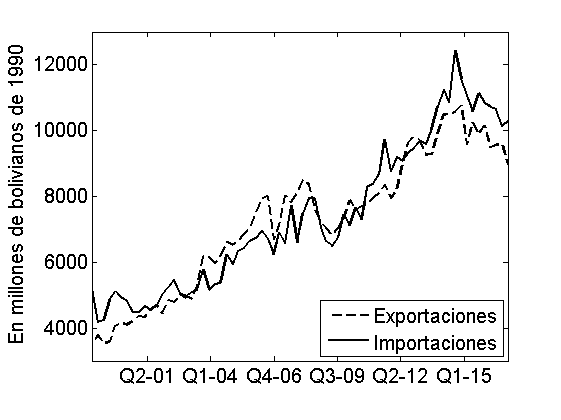
\includegraphics[width=\textwidth]{1xm}
        \caption{Exportación e importación}
        \label{1xm}
    \end{subfigure}
    ~ %add desired spacing between images, e. g. ~, \quad, \qquad, \hfill etc. 
      %(or a blank line to force the subfigure onto a new line)
    \begin{subfigure}[b]{0.3\textwidth}
        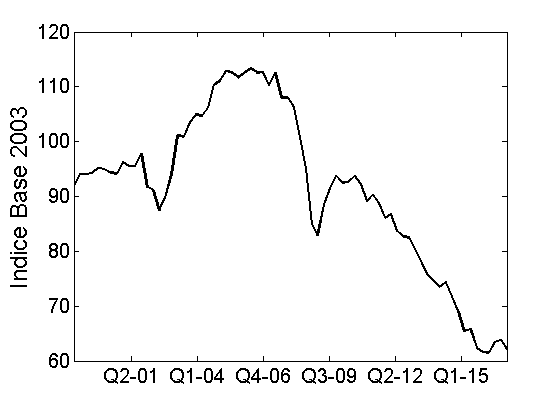
\includegraphics[width=\textwidth]{3tcr}
        \caption{TCR}
        \label{3tcr}
    \end{subfigure}
    ~ %add desired spacing between images, e. g. ~, \quad, \qquad, \hfill etc. 
    %(or a blank line to force the subfigure onto a new line)
    \begin{subfigure}[b]{0.3\textwidth}
        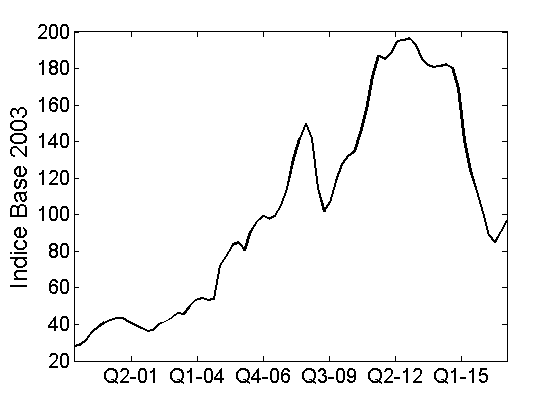
\includegraphics[width=\textwidth]{5ippbx}
        \caption{Precios internacionales}
        \label{5ippbx}
    \end{subfigure}
    \begin{subfigure}[b]{0.3\textwidth}
        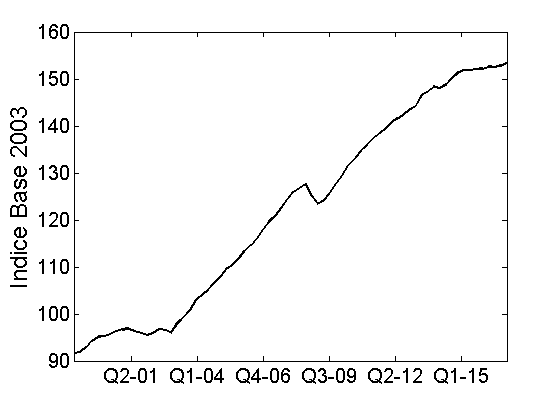
\includegraphics[width=\textwidth]{2per}
        \caption{PIB externo relevante}
        \label{2per}
    \end{subfigure}
    ~ %add desired spacing between images, e. g. ~, \quad, \qquad, \hfill etc. 
      %(or a blank line to force the subfigure onto a new line)
    \begin{subfigure}[b]{0.3\textwidth}
        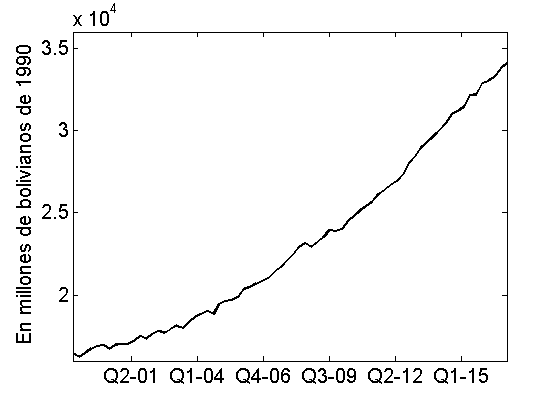
\includegraphics[width=\textwidth]{4pib}
        \caption{PIB}
        \label{4pib}
    \end{subfigure}
\end{figure}

En principio, la verificación gráfica sugiere que las series de importación y exportación comparten tendencia con el producto interno bruto de Bolivia y el de sus principales socios comerciales respectivamente. En el PIB boliviano se advierte una tendencia de crecimiento sostenibilidad desde 1999, sin embargo, desde aproximadamente el 2009, esta presenta una aceleración que dura hasta 2013. El índice del PIB de los socios comerciales más importantes de Bolivia muestra una recesión en 2008 marcada por la crisis financiera internacional y un desaceleramiento a partir de 2013. Esta última variable parece reflejar mejor la tendencia del comercio internacional boliviano. A pesar de que la serie del tipo de cambio real no parece presentar una relación en tendencia tan evidente como la señalada previamente el índice de precios de productos bolivianos exportados parece ser otra serie que captura los ciclos de las exportaciones.

\begin{table}
\caption{Matriz de correlación}
\begin{center}
\begin{threeparttable}
\begin{tabular}{lcccccc}									
\hline													
\hline												
	&	Exportaciones	&	Importaciones	&	PIB externo	&	TCR	&	IPPBX	&	PIB	\\
\hline													
Exportaciones	&	1	&		&		&		&		&		\\
Importaciones	&	0.9384	&	1	&		&		&		&		\\
PIB externo	&	0.9424	&	0.9751	&	1	&		&		&		\\
TCR	&	-0.5185	&	-0.7131	&	-0.7103	&	1	&		&		\\
IPPBX	&	0.8949	&	0.8506	&	0.8743	&	-0.3589	&	1	&		\\
PIB	&	0.9017	&	0.9645	&	0.9835	&	-0.8102	&	0.7821	&	1	\\
\hline													
\hline									
\end{tabular}							
\begin{tablenotes}
\small
\item Elaboración propia.
\end{tablenotes}	
\end{threeparttable}
\end{center}
\label{Rec}	
\end{table}	

Para verificar el análisis gráfico se calcula la matriz de correlación de las variables previamente señaladas. Como había sido adelantado, el PIB externo relevante es la variable más fuertemente asociada a las exportaciones e importaciones seguidas por PIB boliviano y el índice de precios de exportaciones que, como era de esperar, está más correlacionado con las exportaciones. Por otro lado, el tipo de cambio real presenta una correlación negativa con ambas variables especialmente con las importaciones. De acuerdo a la teoría se esperaría que los signos en las ecuaciones \ref{X} y \ref{M} se cumplan y la correlación con las exportaciones sea positiva.

\begin{table}
\caption[Table caption text]{Regresiones de Comercio}
\begin{center}
\begin{threeparttable}
\begin{tabular}{lcccc}									
\hline									
\hline	
	&	(1)	&	(2)	&	(3)	&	(4)	\\
	&	$X$	&	$\Delta x$	& $M$	&	$\Delta m$	\\
\hline	
$y^*$	&	1.700***	&		&		&		\\
	&	(0.035)	&		&		&		\\
$\Delta y^*$	&		&	1.135*	&		&		\\
	&		&	(0.626)	&		&		\\
$y$	&		&		&	1.008***	&		\\
	&		&		&	(0.020)	&		\\
$\Delta y$	&		&		&		&	1.018	\\
	&		&		&		&	(0.353)	\\
$tcr$	&	0.155***	&	&	-0.276***	&	\\
	&	(0.037)	&	&	(0.044)	&	\\
$\Delta tcr$	&	&	0.499**	&	&	-0.095	\\
	&	&	(0.212)	&	&	(0.075)	\\
\hline									
\hline									
\end{tabular}	
\begin{tablenotes}
\small
 \item  \emph{Nota.} La significancia al uno, cinco y diez por ciento es indicada por ***, ** y *, respectivamente.
\end{tablenotes}								
\end{threeparttable}					
\end{center}
\label{Rec}	
\end{table}	

En el cuadro \ref{Rec} se resume los resultados de las regresiones de comercio, se ensayan dos regresiones lineares por cada componente, primero en niveles y después en diferencias. Los resultados en niveles, como es de esperarse, al compartir tanto exportaciones e importaciones tendencia con el PIB externo y el nacional respectivamente se encuentran resultados bastante significativos, pero ``mal especificados'' porque las variables están integradas. Sin embargo, son los resultados de este modelo que realmente miden las elasticidades las cuales no difieren tanto de sus contrapartes diferenciadas. El ensayo de resultados con las variables sin tendencia arroja resultados similares pero menos significativos a pesar de cumplir con las condiciones que la teoría econométrica requiere, sin embargo, demuestran que la relación no es necesariamente espúrea aunque el comportamiento de las importaciones parece estar explicado por otros determinantes. Asimismo, es importante destacar es la que las variables son elásticas a las variables de producción, sin embargo, bastante inelásticas al tipo de cambio real.

\begin{figure}
\centering
\caption{Estructura de importaciones y exportaciones de Bolivia}\label{impexp}
    \begin{subfigure}[b]{0.75\textwidth}
        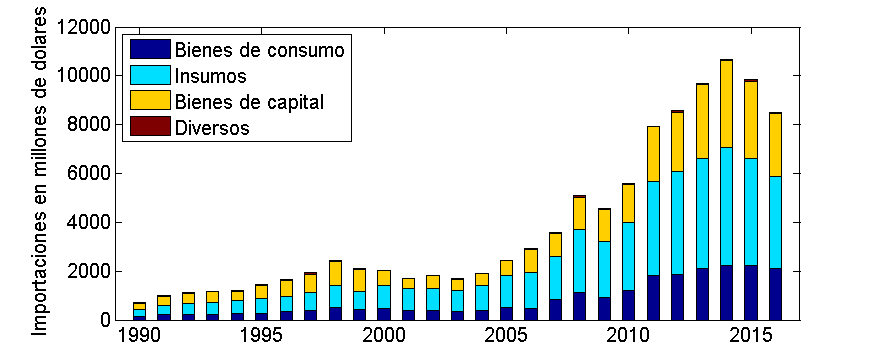
\includegraphics[width=\textwidth]{imp9016}
        \caption{Estructura de importaciones}
        \label{mestr}
    \end{subfigure}
    \begin{subfigure}[b]{0.75\textwidth}
        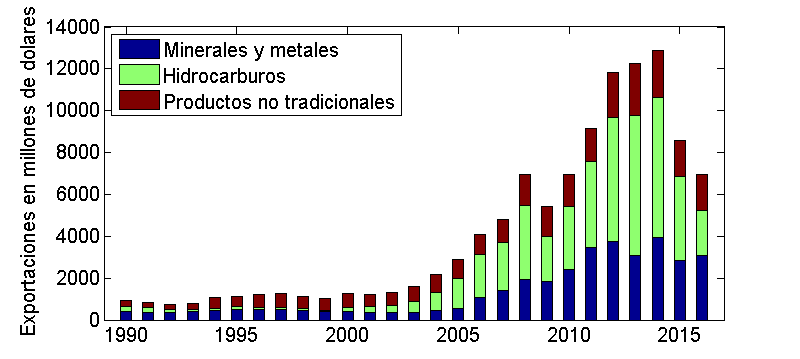
\includegraphics[width=\textwidth]{exp9016}
        \caption{Estructura de exportaciones}
        \label{xestr}
    \end{subfigure}
\end{figure}

La explicación a este fenómeno es interesante y depende de las características particulares del comercio externo boliviano. Las exportaciones bolivianas se componen en promedio 78\%, desde la nacionalización de hidrocarburos en Bolivia en 2007, en materias primas cuyos precios están definidos en los mercados internacionales, donde el pequeño tamaño del comercio boliviano no tiene influencia en la determinación del precio. La exportación de materias primas bolivianas, al tener el mismo precio en todos los países, generalmente en dólares, no son influenciadas por el tipo de cambio real. A priori se estima que por construcción esta variable solo tendría una influencia con las manufacturas que son exportadas por la industria boliviana, la cual es de una proporción mucho menor, en especial si se la compara, por ejemplo, con el gas y los minerales exportados. Al mismo tiempo, tanto los minerales como la mayoría de los productos no tradicionales tienen precios fijados en los mercados internacionales. Las manufacturas oscilan en participación entre 12-25\% entre 1999 y 2006 y 7-12\% en 2007-2016 siendo este último periodo en el que el volumen exportado de manufacturas se llegó a triplicar. 

Por el lado de las importaciones, se nota que la estructura se mantiene similar a través de los años a pesar del incremento notable suscitado en 2004 y confirmado en 2005. Acerca de la inelasticidad de las importaciones con respecto al tipo de cambio real se pueden plantear varias hipótesis de carácter general que la explicarían.
\begin{itemize}
\item La pequeña industria boliviana no alcanza para satisfacer la demanda boliviana de bienes por lo que las importaciones son precio inelásticas. Al mismo tiempo, no existen productos domésticos para sustituir a las importaciones.
\item El precio de los bienes bolivianos es muy elevado, por lo que se prefieren los precios más bajos importados incluso frente a un tipo de cambio muy devaluado. Esto podría ser ocasionado por el uso de tecnologías domésticas atrasadas o caducas que hacen que los precios domésticos sean más elevados. Por otro lado, los precios más bajos debido al contrabando juegan un papel muy importante en este sentido.
\item La calidad de los bienes importados es superior a la producción doméstica. Esto podría deberse a que la tecnología doméstica es atrasada o que el costo de producir mayor calidad es muy elevado. Por otro lado, relacionando esta hipótesis con la previa se puede pensar que el precio doméstico no es acorde a la calidad ofrecida por lo que la demanda de bienes importados es inelástica al tipo de cambio real. 
\end{itemize}

De todas maneras, del Cuadro \ref{Rec} se rescata que el comercio externo es muy sensible al rendimiento de las economías extranjeras, y en el caso de las importaciones al de la economía doméstica. La baja sensibilidad al tipo de cambio real implica que sería necesario cambios muy elevados de este para generar variaciones significativas en el comercio externo boliviano. Las elasticidades estimadas son utilizadas para calcular la ecuación \ref{r}, en el que se utilizan los valores tendenciales de demanda doméstica, demanda externa y precios de exportaciones.

Posteriormente se estima la varianza de la variación estimada y se hace la medición para encontrar el valor de equilibrio del tipo de cambio real.

\begin{figure}
\caption{Resultados DEER}
\centering
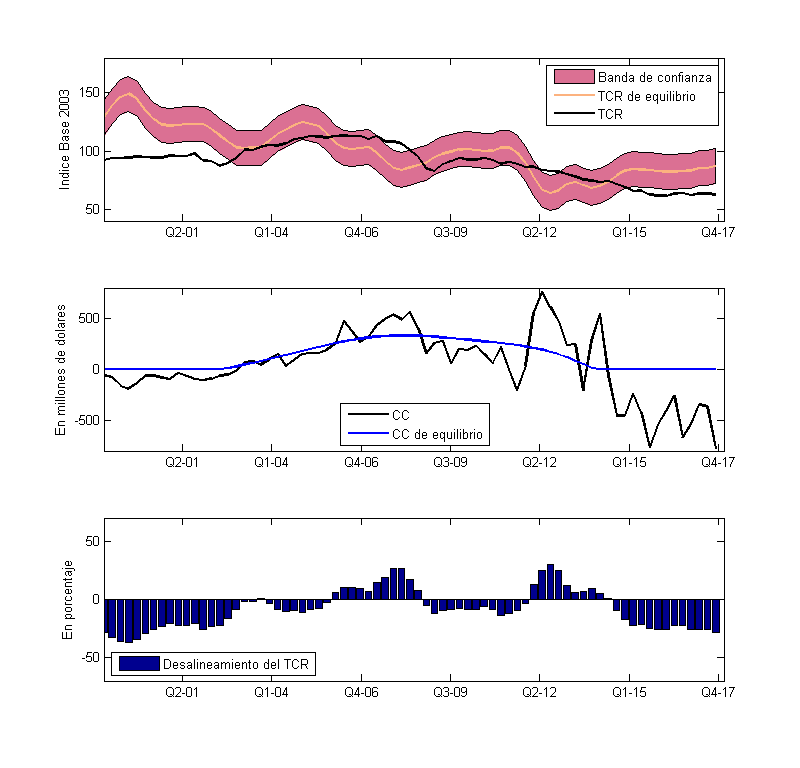
\includegraphics[scale=0.75]{tcreq}
\end{figure}

De esta evidencia se verifica que el tipo de cambio real estuvo desalineado durante dos periodos de la muestra planteada. A partir del 2006 la diferencia entre el tipo de cambio real observado y de equilibrio tiende a ser mucho menor. A partir del 2014 la divergencia de ambas series comienza a ser fuerte. En estos periodos de desequilibrio se entiende que el tipo de cambio real se encontraba sobre valuado. Es decir que para restaurar el equilibrio era necesario devaluar el boliviano. En efecto, si verificamos paralelamente a los tipos de cambio reales observados y de equilibrio junto con la cuenta corriente observada y de objetivo podemos verificar que los desalineamientos en tipo de cambio coinciden con los de cuenta corriente. 

Desde esta óptica, es importante verificar que la mayor variación de cuenta corriente correspondiente a 2013 y la tendencia a la baja ya eran indicios importantes para que gestionar la política que pueda generar la depreciación del tipo de cambio real para poder conseguir el equilibrio externo y evitar los déficits incurridos.

Es importante notar que las variaciones de tipo de cambio son un tema particularmente delicado en Bolivia por la historia inflacionaria y el hecho que la economía está anclada nominalmente al valor del dólar. Por otro lado, al ser las exportaciones dependientes del precio de las materias primas que comercia internacionalmente un buen indicador de la dirección que la balanza comercial, y por ende, la cuenta corriente vayan a tomar son los precios de materias primas exportadas. Ceteris paribus se puede calcular cual es la medida en la que el tipo de cambio nominal debería ser depreciado para mantener un equilibrio con cuenta corriente no deficitaria.

Otro punto interesante de estos resultados se enfoca en el periodo previo a 2006. El mismo implica que durante la época neo liberal el tipo de cambio real no estuvo alineado con sus valores de equilibrio a pesar de depreciar el tipo de cambio nominal en función al tipo de cambio referencial que supuestamente  mantiene el tipo de cambio real constante y competitivo. Por lo menos, la cuenta corriente y balanza comercial se encontraron en déficit sostenidos, lo cual bajo ningún concepto se traducen a niveles de equilibrio de tipo de cambio.

\footnote{Si bien esto es cierto, en la realidad los bienes primarios transados bilateralmente entre países tienen como precio aplicable aquel pactado en los contratos suscritos entre partes, el cual puede ser o no el mismo que los determinados por los mercados internacionales, tal vez debido a otros factores como la calidad o el costo de transporte u otras consideraciones. Sin embargo, y sin lugar a dudas estos precios internacionales son el referente de los precios últimos contratados por materias primas.}	






\subsection{BEER}
%datos
Previa a la estimación, la especificación adoptada en la sección anterior requiere la construcción u aproximación de algunas de las variables denominadas como fundamentos. 
Para el caso de la productividad, se plantean tres medidas alternativas para su aproximación, i. Se construye un ratio entre el PIB percápita  de Bolivia y el de sus socios comerciales, para tal efecto se considera  frente La medición de la productividad variables La estimación del modelo se realiza a partir de un modelo de cointegración. Como se ha explicado más arriba la razón se basa en la relación de largo plazo que se encuentra entre las variables especificadas en \ref{qb}, complementariamente, el modelo de corrección de errores propone un las variaciones de corto plazo del modelo.

Vale la pena considerar que este tipo de modelos siempre presentará resultados que muestran que los datos observados parecen estar alrededor de la tendencia y dentro de las bandas de confianza del modelo. Esto porque básicamente el modelo de cointegración está usando los datos observados de tipo de cambio real y está calculando el modelo alrededor de ellos. Por tal motivo, no se verá divergencias grandes de la tendencia.

Sin embargo, lo particular de estos modelos son las variaciones que existen a un nivel de menor frecuencia, es decir los altos y bajos picos que puedan surgir que muestran el desequilibrio del modelo.
%graficos




\section{Consideraciones Preliminares}\label{consid}


\subsection{Movimientos del tipo de cambio real}
Debido a que la fórmula de tipo de cambio real es la definida por \ref{tcr1} o \ref{tcrlog} y el tipo de cambio nominal es el principal instrumento de la política cambiaria, se hace tentador simplemente despejar esta variable de la fórmula para que ella indique cual, para el nivel deseado de tipo de cambio real, es el nivel de depreciación nominal necesario para lograr el nivel de TCR definido. Este es el método mediante el cual se encuentra el tipo de cambio referencial al que se hace mención en la introducción de este documento. Sin embargo, el uso de esta estrategia puede ser considerado una falacia teórica.

La razón es porque, en contraposición de los precios extranjeros que son exógenos, los precios de la economía doméstica dependen, o están en función entre otras cosas, del tipo de cambio nominal $p(e)$. Al respecto, la evidencia más grande está en la literatura de \emph{pass-through} de tipo de cambio a inflación, la cuál generalmente obtiene valores distintos de cero y positivos. El hecho que el coeficiente de \emph{pass-through} sea distinto de cero implica que la depreciación del tipo de cambio nominal, desde una perspectiva de instrumento, genera presiones en el nivel de precios hacia el alza. Entonces, tanto el tipo de cambio nominal como el nivel de precios se incrementan determinando que en el corto plazo el efecto de una devaluación nominal se aminore.

En la realidad existen dos factores empíricos importantes que matizan esta situación. El efecto \emph{pass-through} no se da inmediatamente debido a la rigidez de precios, es decir que la transmisión del incremento del tipo de cambio a los precios no ocurre inmediatamente sino a medida que los precios se reajustan a dicho cambio, únicamente una economía con total flexibilidad de precios o indexada perfectamente a la divisa de referencia transmitiría inmediatamente dicho efecto. Por otro lado, es un caso muy extremo cuando el parámetro \emph{pass-through} llegue a ser unitario pues implicaría que no solamente el sector transable es perfectamente sensible sino también el sector no transable lo es, en cuyo caso se podría pensar que el tipo de cambio afecta a los costos importados de bienes no transables. Otra probable explicación es que el efecto en los precios transables y no transables sobre-reaccionen debido a las expectativas inflacionarias y/o devaluativas haciendo que el efecto total de \emph{pass-through} llegue a la unidad, lo cual implicaría que la economía se encuentra en una posición demasiado riesgosa.

Otra consideración importante es que el nivel de \emph{pass-through} es variable, es decir que no es fijo a través del tiempo si no que depende de la situación particular en el que cada economía esté. Esto probablemente debido a la formación de las expectativas de los agentes. Por tanto, el uso adecuado del tipo de cambio nominal es complicado y sensible a varias consideraciones.

En el caso de Bolivia, el uso de la regla cambiaria siguiendo el tipo de cambio de referecia, es decir  utilizando la estrategia previamente mencionada, mientras estuvo vigente el \emph{crawling peg} no se logró la fijación del tipo de cambio real en el valor deseado. Durante el periodo en el que este régimen estuvo vigente el tipo de cambio real se situó volátilmente bajo su meta y durante 1994 y 1995 por encima de ella, mientras que la constante depreciación buscaba y suponía lograr el valor deseado puntualmente en cada periodo.

En realidad, lo que demuestra el comportamiento durante 1990 y 2003 es que la velocidad de la depreciación es menor que el de los precios internos dado el ajuste al nivel de precios externos exógenos. Potencialmente, esto implicaría que la aceleración de la depreciación generaría una velocidad aún mayor en el nivel de precios local. Esto implica que no se logra tomar en cuenta el efecto inflacionario de la devaluación en el nivel de precios locales. En particular, el desajuste entre 1994 y 1995 se debe principalmente al repunte inflacionario de Brasil, uno de los principales socios comerciales de Bolivia que en estas fechas introduce el real como moneda oficial, este factor externo originó que la moneda boliviana se deprecie más de lo esperado en términos reales. Al mismo tiempo, este evento se constituye en un shock que marca la leve desaceleración de la depreciación boliviana que no es tan pronunciada como la sugerida por su tipo de cambio referencial.

Es posible que la moderada depreciación y el anclaje de la expectativas de los agentes en la misma depreciación colaboró a que la inflación importada de Bolivia no sea incluso más elevada. Sin embargo, este hecho demuestra empíricamente la falacia teórica acerca de como mover el tipo de cambio real con su parte nominal.











\section{Conclusiones}\label{concl}

Los modelos muestran que bajo el objetivo de sostenibilidad externa utilizado los mayores desajustes corresponden a los periodos en los que la cuenta corriente se encuentra en desequilibrio principalmente por los déficits en balanza comercial. Al mismo tiempo, estos periodos coinciden con aquellos en los que los precios de materias primas no fueron lo suficientemente beneficiosos para el esquema comercial internacional boliviano.

A pesar de que hasta 2004 se siguió una regla cambiaria que buscaba determinar al tipo de cambio real en un nivel fijo de competitividad, la evidencia muestra que esta política falló fuertemente, pues no consideró que al depreciar el tipo de cambio nominal, este se contrarrestaría con el movimiento de la inflación determinado por el efecto \emph{pass-through}, este es sólo uno de los motivos por los que esta regla cambiaria no funcionó para conservar un nivel estable de tipo de cambio real, Rodrik menciona otro, la falta de capacidad para generar ilusión monetaria. Al mismo tiempo, las mini-devaluaciones solamente sirvieron para ayudar un pequeño grupo de exportadores de manufacturas, mientras que hacía que las importaciones se encarecieran constantemente en términos de la moneda boliviana, esta es la raiz de una sostenida inflación importada y de la dolarización de ese periodo debido a que las expectativas cambiarias de la población estaban ancladas en la depreciación.

Durante el boom de los precios de materias primas y muy en especial después de la nacionalización de hidrocarburos en Bolivia el 2006 se vivió el recuperamiento de la balanza comercial dado que la mayoria de las exportaciones eran el gas vendido a Brasil y Argentina. Este hecho representó una gran entrada de divisas a la economía que fortaleció a las RIN y dotó de suficientes dólares americanos para cubrir los requerimientos de los mismos en el mercado interno. La apreciación real de la moneda significó que en este periodo de auge económico sea conveniente importar bienes. Por otro lado, el ancla nominal cambiaria se fijó en la estabilidad del boliviano. Este hecho contribuyó a la des-dolarización de la economía.

Finalmente, después de la caída de precios internacionales de materias primas, la economía boliviana logró sobrevivir por la solidez ganada en periodos previos y los aún significativos ingresos de hidrocarburos. Sin embargo, la cuenta corriente se vio afectada así como las RIN. Si bien durante este periodo la opinión pública reclamó una depreciación se considera que por la evidencia expuesta previamente, esta medida no podría haber podido cumplir el fin deseado de nivelar de nuevo la balanza comercial debido a que el volumen de la exportación de gas y minerales no dependen de esta variable.

Como se ha visto, la estabilidad cambiaria tiene gran aporte en la des-dolarización de la economía, sin embargo, el gobierno boliviano no ha delusidado aún la manera de mantener un tipo de cambio real estable y la evidencia señala que aún está experimentando con los instrumentos que tiene a su disposición. Asimismo, el auge económico respaldado por el comercio internacional fue patrocinado por el incremento de los precios del gas que también coincidió con la apreciación del tipo de cambio real y la débil consecución de la regla cambiaria que posteriormente fue abandonada al encontrar en en la estabilidad un refugio para permitir que la moneda local se fortalezca en el mercado interno que fue beneficiado por bajos precios de importaciones que a su vez beneficiaron a la mayor parte de la población que se dedica a este rubro y que a su vez permitió el crecimiento del sector no transable del país.


Como se ha evidenciado, el tipo de cambio real no es muy influyente para mover la balanza comercial debido a la inelasticidad de sus componentes a esta variable. Sin embargo, se han determinado los periodos en los que, dada la situacón y si el tipo de cambio fuese más flexible, el movimiento del tipo de cambio hubiese mejorado la situación de la economía.


La regla cambiaria utilizada es incorrecta porque no determina la dirección del TCR, este punto ya ha sido probado hace tiempo.


Bolivia necesita entre otras cosas es una industria que produzca transables y no transables sustituibles dentro de la economía y fuera también, sin eso estamos dependiendo fuertemente de los designios de los movimientos de la economía extranjera.

Posibilidad de enfermedad holandesa. no existe porque no hay otro sector que se pueda matar.


Hay que entender que el tipo de cambio real está calculado en base a las variaciones de los índices de precios al consumidor de los socios comerciales y local y de los tipos de cambio. Como se toma en cuenta los índices de precios al consumidor, esta medida captura la variación real de artículos que entran en la canasta básica de consumo de cada país. Es evidente que esta puede diferir entre economías, sin embargo, el cálculo del tipo de cambio real hace abstracción de estas divergencias y asume que son lo suficientemente parecidas. El punto importante que se debe notar es que captura los precios de bienes de consumo interno y que están dentro de la canasta básica, los cuales no son bienes que Bolivia exporta, en contraposición si son bienes que importa. Por este motivo es que la inclusión de los valores 

\bibliography{tcr_bolivia}

\bibliographystyle{humannat}

\end{document}
